
\thispagestyle{empty}

\begin{center}
\Large
%Introduction
Préambule
\normalsize
\end{center}
\vspace{3cm}

Ce document est une compilation d'articles provenant de deux
ouvrages : {\it La pratique de la philosophie} destiné aux
lycéens, une encyclopédie de la philosophie destinée aux néophytes.

%(Complété par un dictionnaire encyclopédique de poche et un
%dictionnaire étymologique pour l'article {\it vérité.})

Il souhaite donner un aperçu élémentaire et succinct de la
philosophie à propos de la religion et des religions.

%\vspace{1.3cm}
\vfill

\begin{center}
%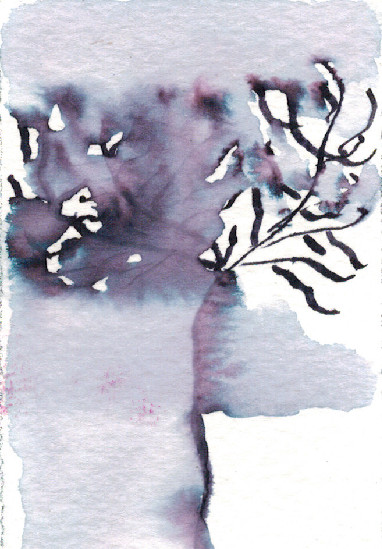
\includegraphics[scale=0.5]{./presentation/gauche2}
\hspace{1cm}
%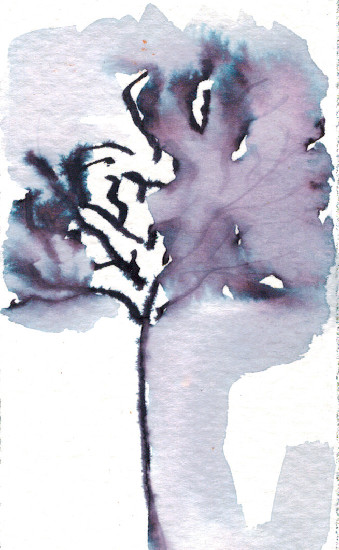
\includegraphics[scale=0.5]{./presentation/droite2}
\end{center}

\vfill
\vspace{1.7cm}

\hfill {\it Les documents de Zécriture}

\hfill \texttt{www.zecriture.fr}

\vspace{0.7cm}


\hfill Numérisation : Stephan Runigo

\hfill Illustrations : Christiane Audhuy

%%%%%%%%%%%%%%%%%%%%%%%%%%%%%%%%%%%%%%%%%%%%%%%%
